% #############################################################################
% This is Chapter 4
% !TEX root = ../main.tex
% #############################################################################
% Change the Name of the Chapter i the following line
\fancychapter{Methodology}
%\cleardoublepage
% The following line allows to ref this chapter
\label{chapter:methodology}

As mentioned earlier, in this work \ac{DL} methods are used to segment fluorescent microscopic images. The first phase is to implement supervised models to accomplish this task of segmenting the nuclei and Golgi of these images. Then we focus on the main goal, which is to implement an unsupervised model that can perform the same task as well or better than the supervised models. And finally, we add a third class to detect the nucleus-Golgi pairs.

This chapter begins by presenting the dataset used to train, validate, and test these models. The proposed approach to semantic segmentation using an unsupervised model is described in Section \ref{section:proposed}. The performance of this approach is compared to the supervised models, which are described in detail in Section \ref{section:comparison}. Then, Section \ref{section:models_inference} describes how the models are used for inference after training. Finally, Section \ref{section:execution_time} describes how the training and testing time of the models is determined to be used as a measure of the performance of the different approaches.

\section{Dataset}
\label{section:dataset}

The dataset used in this work consists of eight crops extracted from \ac{3D} fluorescence microscopy images of mouse retinas. These crops range in size from 257x505x55 to 627x818x61. In these crops, the nuclei are labeled with green fluorescent protein (GFP) and the Golgi are labeled with mCherry. In addition, manually labeled segmentation masks are used for training the proposed supervised methods and evaluating their performance. These masks are RGB, with the red channel containing the segmentation mask of the Golgi and the green channel containing the segmentation mask of the nuclei. The blue channel contains the segmentation mask of the nucleus-Golgi pairs, but only for the task of the 3-class segmentation problem. In this case, the input images and the output masks have 3 channels. For the 2-class segmentation problem, the blue channel is not considered, so the input images and the output masks have only two channels (these masks are converted to RGB for visualization but the blue channel is all zeros).

An example of a \ac{3D} crop and its corresponding manually labelled segmentation masks for the 2-class task and 3-class task can be found in Figure \ref{fig:dataset_original}.

\begin{figure}[!htb]
	\centering
	\subfigure[]{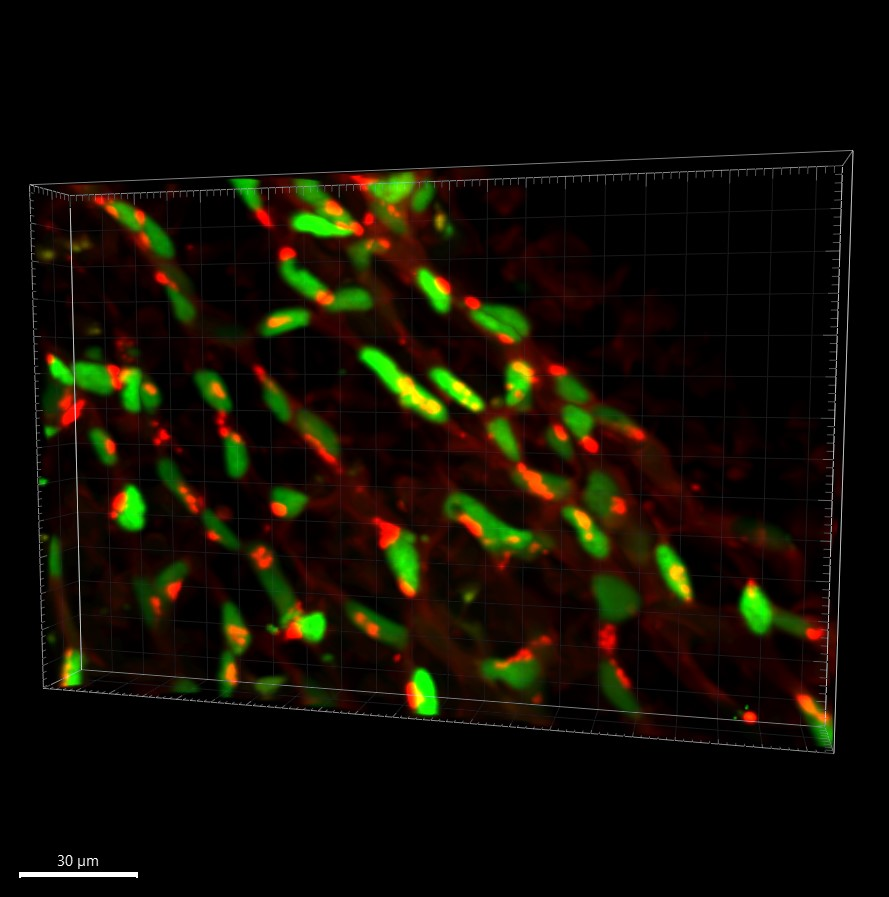
\includegraphics[width=4.5cm]{Images/img_crop1.jpg}}\hfil
  \subfigure[]{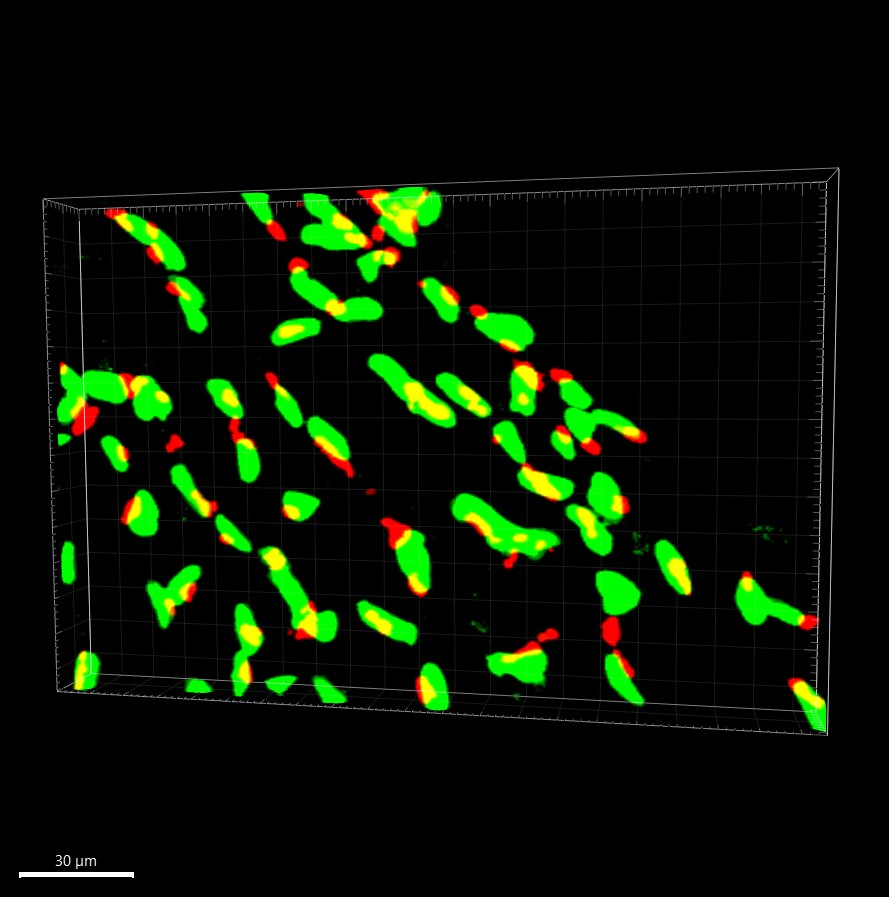
\includegraphics[width=4.5cm]{Images/mask2_crop1.jpg}}\hfil 
  \subfigure[]{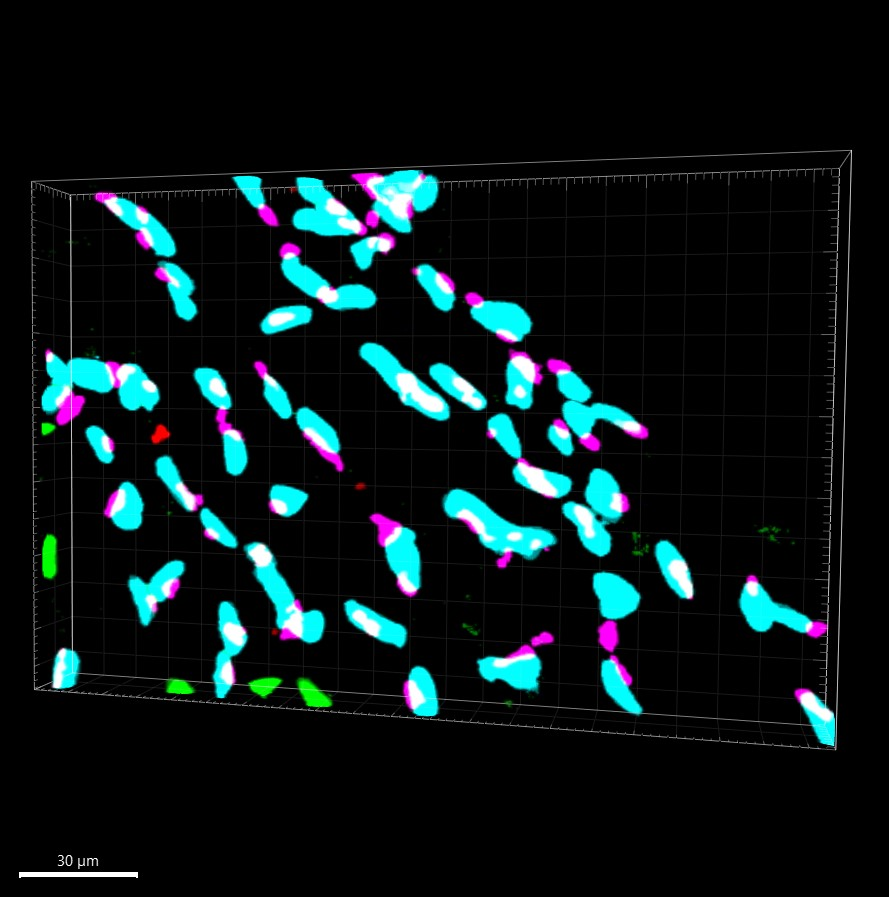
\includegraphics[width=4.5cm]{Images/mask3_crop1.jpg}} 
	\caption[(a) Example of a 3D crop of a microscopy image of mouse retina; (b) 3D ground truth mask for 2-class task; (c) 3D ground truth mask for 3-class task.]{(a) Example of a \ac{3D} crop of a microscopy image of mouse retina; (b) \ac{3D} ground truth mask for 2-class task; (c) \ac{3D} ground truth mask for 3-class task.}
	\label{fig:dataset_original}
\end{figure}

To use these crops to train the models, its necessary to divide them into equal sized patches. If the volumes are too small, not enough information can be learned. If the volumes are too large, training will take longer and could exceed GPU memory. Therefore, we set the size of these patches to 64x64x64. Since the $z$-axis of the original images has a size between 55 and 61, the crops had to be padded to get the 64 slices in the $z$-axis for the input images, for this purpose a reflection padding was applied.

\subsection{Synthetic segmentation masks}
\label{subsection:synthetic_masks}

As mentioned earlier, the manually labelled segmentation masks are used for training the implemented supervised models. However, in order to train the proposed model in a non-supervised way, synthetic segmentation masks had to be created. 

For this purpose, ellipsoids are created to represent the nuclei and spheres for the Golgi at random positions. For each nucleus-Golgi pair created, the radius of the spheres (nucleus) and the size of the principal and secondary axis of the ellipsoids (Golgi), the distance between the nucleus and Golgi (relative to the center of the Golgi), and the rotation of each pair are selected randomly from the intervals [5,9] pixels, [[17,30],[8,13],[8,13]] pixels, [-6,6] pixels and [0,180] degrees, respectively. For each crop created, a random number of nucleus-Golgi pairs were selected (between 45 and 70 pairs). To make the images more realistic, an elastic transformation was applied to each nucleus-Golgi pair. This transformation consists in deforming the image using displacement vectors and a spline interpolation. The value of this displacement is set to 0.75. Six crops were created with the same size of the six microscopic image crops used for training the model. An example of a synthetically created segmentation mask can be found in Figure \ref{fig:sintetica} (a).

For the 3-class segmentation problem, another six synthetic segmentation masks were created to train the models for this task. Here, the nuclei and Golgi are generated in the same way as described previously. In this case, a third segmentation mask is added in the blue channel corresponding to the class of the nucleus-Golgi pairs that corresponds to the union of the nuclei and Golgi generated for the green and red channels, respectively. To make the images more realistic, isolated nuclei and Golgi are added to the segmentation mask and are not included in the segmentation mask of the nucleus-Golgi pairs (blue channel). An example of a synthetically generated segmentation mask can be found in Figure \ref{fig:sintetica} (b).


\begin{figure}[!htb]
	\centering
	\subfigure[]{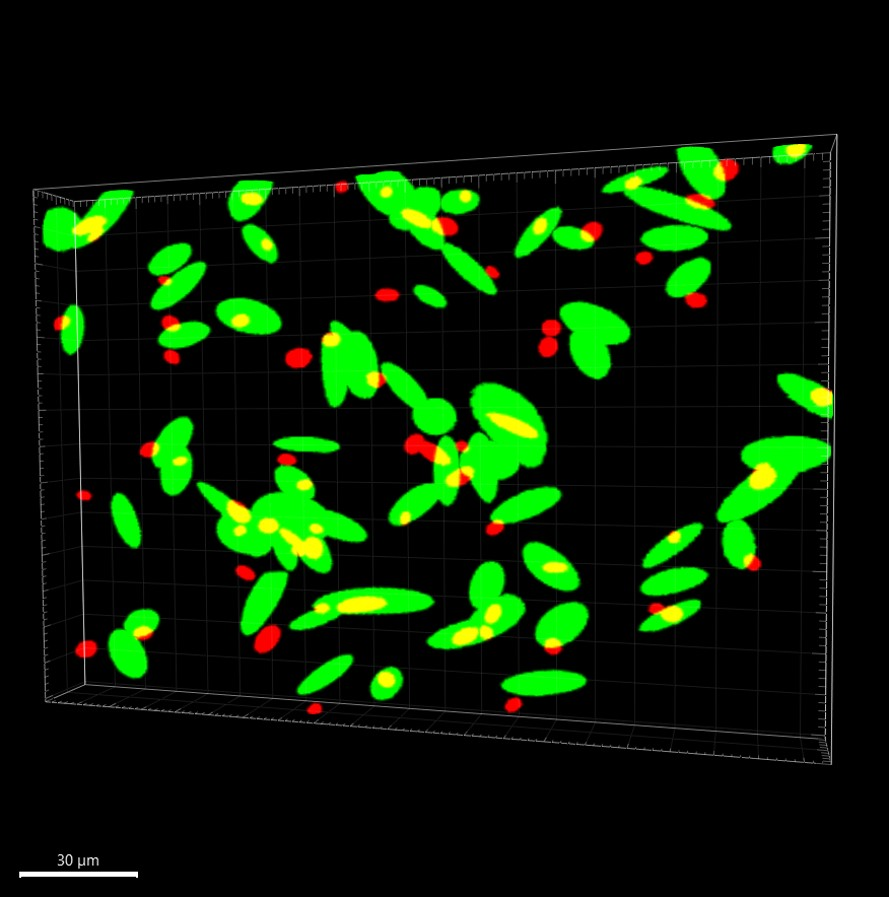
\includegraphics[width=5cm]{Images/2-mask-synthetic.jpg}}\hfil
  \subfigure[]{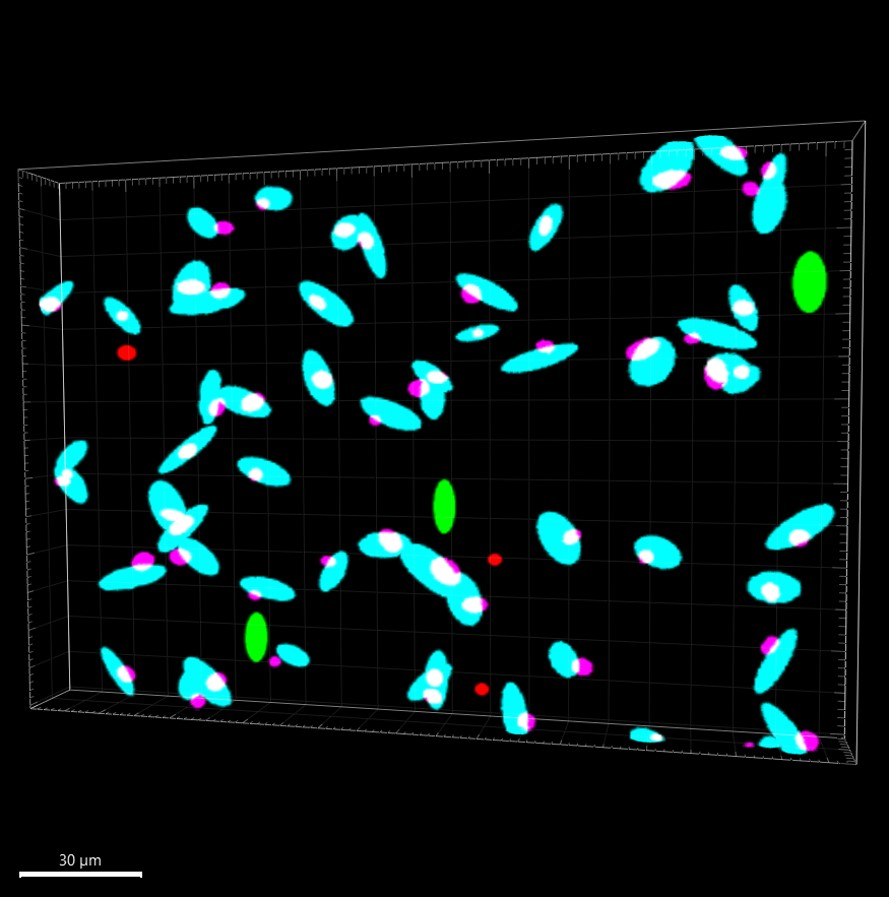
\includegraphics[width=5cm]{Images/3-mask-synthetic.jpg}}
	\caption[Example of synthetic 3D segmentation masks for: (a) 2-class segmentation task; (b) 3-class segmentation task.]{Example of synthetic \ac{3D} segmentation masks for: (a) 2-class segmentation task; (b) 3-class segmentation task.}
	\label{fig:sintetica}
\end{figure}


\section{Proposed Approach}
\label{section:proposed}

For this work, cell nuclei and Golgi semantic segmentation will be performed using the cycle-consistent GAN model, CycleGAN for short. Two different domain images will be considered, the fluorescence microscopy images (domain $I$) and the synthetic segmentation mask (domain $S$). Moreover, let $i$ and $s$ denote training examples where $i \in I$ and $s \in S$.

Like the original CycleGAN model \cite{cycleGAN:original}, the architecture of this segmentation model will be composed of four interconnected networks, two generators and two discriminators. A representation of this network can be found in Figure \ref{fig:diagrama}. The first generator ($G_S$), corresponding to the segmentation network we wish to obtain, learns a mapping from the domain $I$ to $S$. The first discriminator ($D_S$) takes the segmentation masks as input and tries to predict whether they are real or generated, according to the domain $S$. In contrast, the second generator ($G_I$) learns a mapping from the domain $S$ to $I$, and is used only to improve the training. Furthermore, the second discriminator ($D_I$) receives an image as input and predicts whether this image is real or generated, according to domain $I$.

\begin{figure}[!htb]
  \centering
  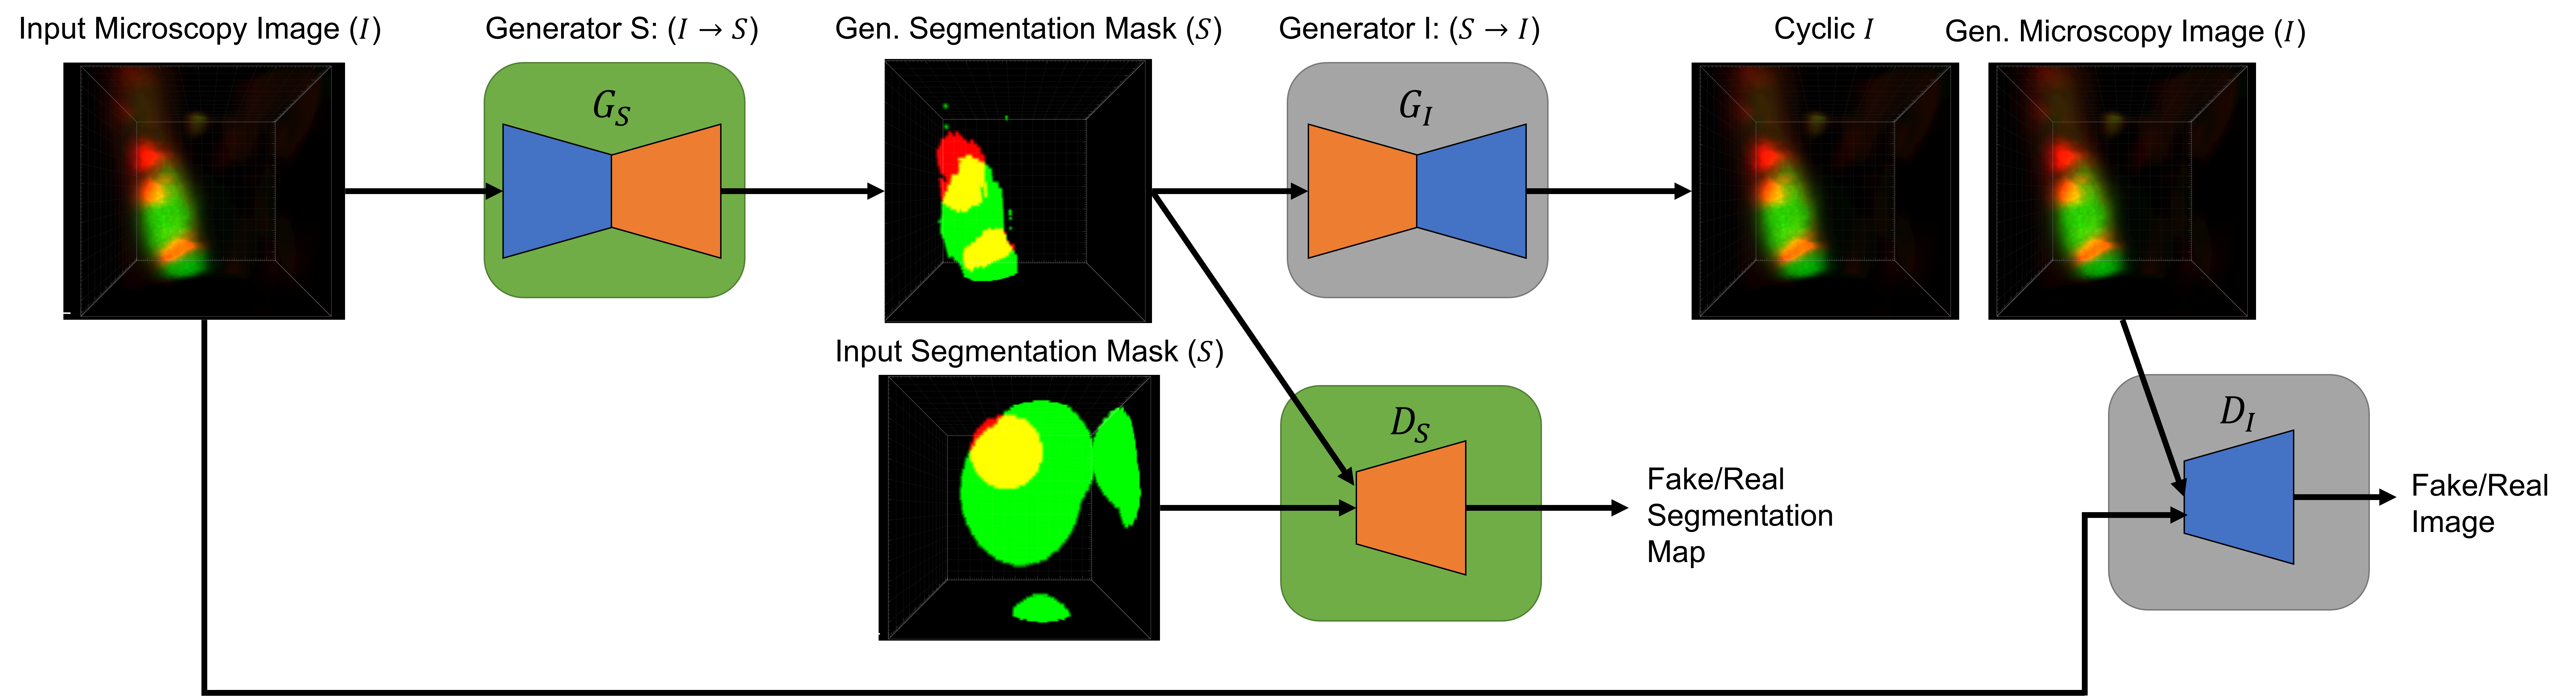
\includegraphics[width=0.99\textwidth]{Images/diagrama.jpg}
  \caption[CycleGAN schematic for the proposed approach.]{CycleGAN schematic for the proposed approach.}
  \label{fig:diagrama}
\end{figure}


\subsection*{Network Architecture}

The generator architecture used in the original CycleGAN model is intended for a \ac{2D} image-to-image translation task. Therefore, for our dataset, this approach needs to be adapted to perform a \ac{3D} image-to-image translation. This can be achieved by replacing the \ac{2D} convolutional layers of the original CycleGAN with \ac{3D} convolutional layers.  The discriminator architecture to be implemented is based on the PatchGAN \cite{isola2018imagetoimage}, which includes \ac{Leaky ReLU} for nonlinearity. The layers of the discriminator architecture must also be converted from \ac{2D} to \ac{3D}. The detailed architecture of the generator and discriminator used in the CycleGAN model employed in this work are shown in Figures \ref{fig:gencyc} and \ref{fig:disccyc}, respectively.

\begin{figure}[!htb]
  \centering
  
\includegraphics[width=0.99\textwidth]{Images/generator_cyclegan.jpg}
  \caption[Implemented CycleGAN generator architecture. The Residual Block consist of a 3D convolutional layer with instance normalization and ReLU as the activation function, followed by a second convolutional layer also with instance normalization. The output of this block is the concatenation of the output of the second layer with the input layer of the block. $k=(x,y,z)$ denotes the size of the input image for the x, y and z axes.]{Implemented CycleGAN generator architecture. The Residual Block consist of a \ac{3D} convolutional layer with instance normalization and \ac{ReLU} as the activation function, followed by a second convolutional layer also with instance normalization. The output of this block is the concatenation of the output of the second layer with the input layer of the block. $k=(x,y,z)$ denotes the size of the input image for the x, y and z axes.}
  \label{fig:gencyc}
\end{figure}

\begin{figure}[!htb]
  \centering
  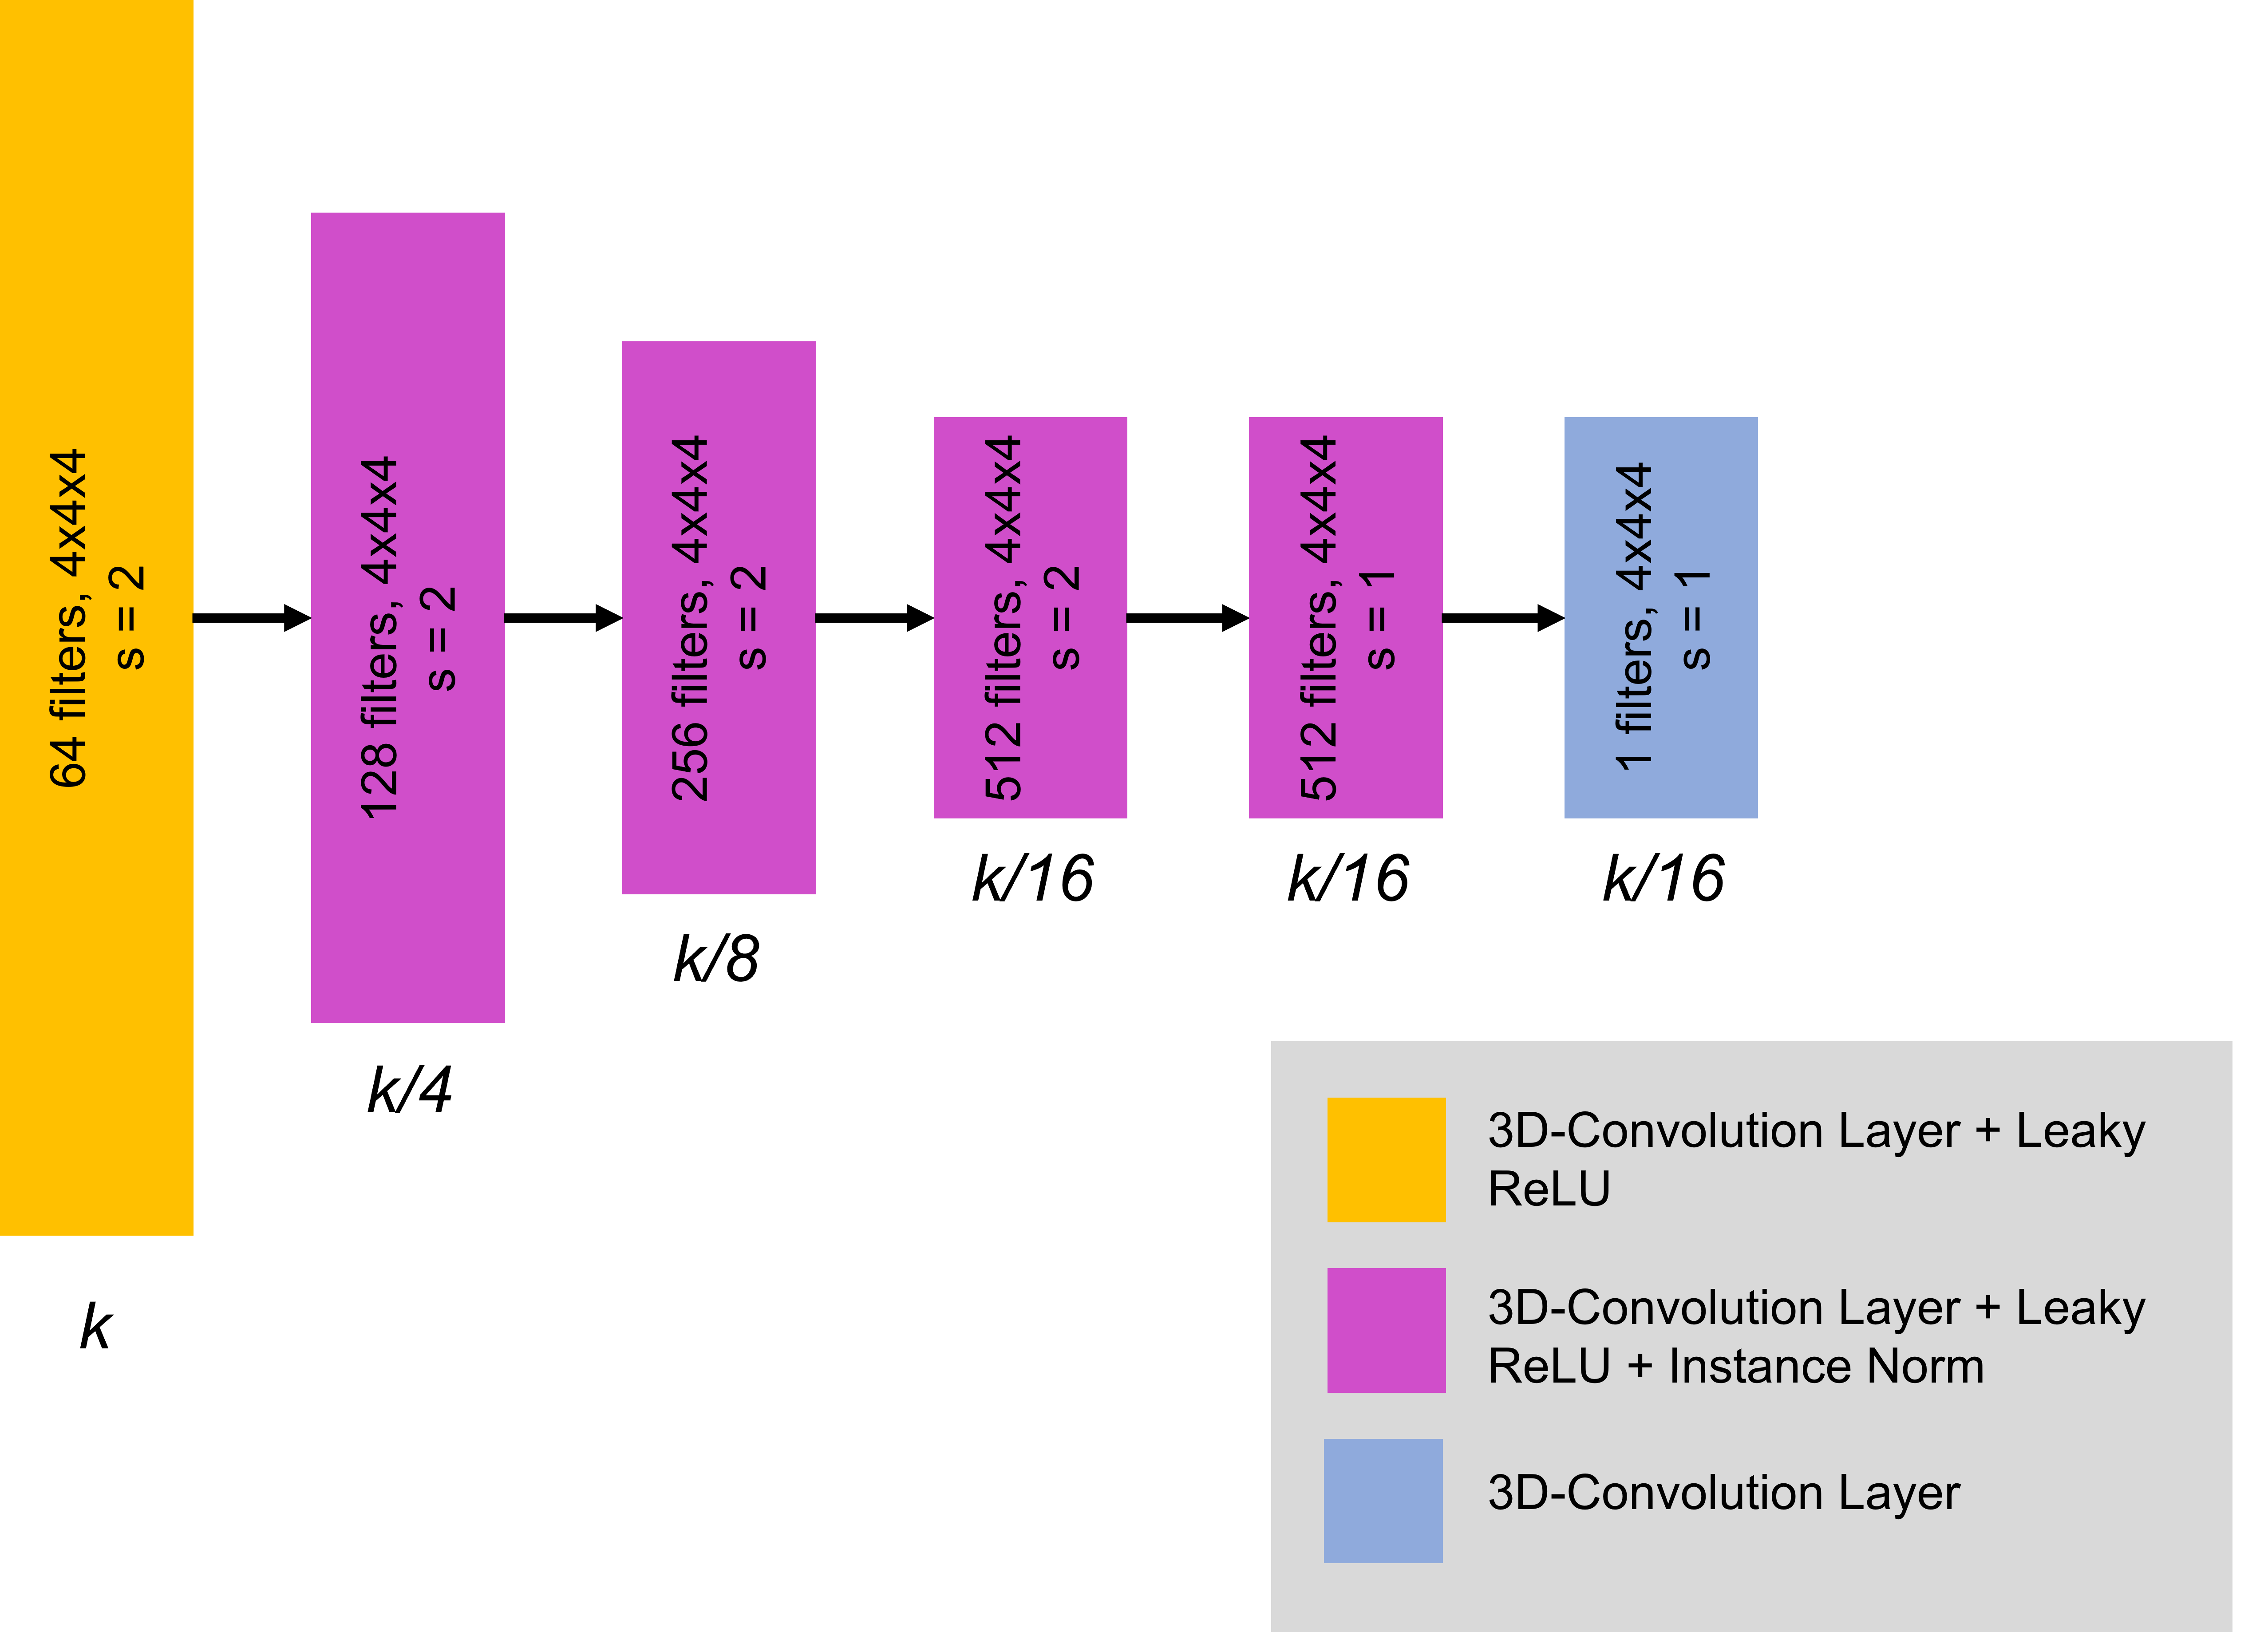
\includegraphics[width=0.50\textwidth]{Images/discriminator_cyclegan.jpg}
  \caption{Implemented CycleGAN PatchGAN discriminator architecture. $k=(x,y,z)$ denotes the size of the input image for the x, y and z axes.}
  \label{fig:disccyc}
\end{figure}

In the Figures \ref{fig:gencyc} and \ref{fig:disccyc} above, each box corresponds to a convolution block in the model. For each block, the type of convolutional layer and the normalization and activation function used after each layer are described in the Figure legend. The size of the feature map that each convolution block outputs is provided at the bottom of the boxes with respect to the size of the input image $k$. In each box, the number of filters, the size of these filters, and the stride used in each convolutional layer are indicated.

\subsection*{Loss functions}

The loss function used to train CycleGAN comprises four terms. These terms are described below.

\textbf{Adversarial Loss.} The adversarial term encourages the mapping functions to translate from one domain to
the other. First, the negative log likelihood objective from $\mathcal{L}_{GAN}$  (Equation \ref{eq:GAN}) is replaced by a least-squares loss, since according to \cite{cycleGAN:original}, this loss is more stable during training and produces higher quality results. Therefore, the adversarial loss for the first GAN ($G_{S}, D_S$), for the already mentioned notation, is given by,

\begin{equation}
    \mathcal{L}_{adv}(G_{S},D_S) = \mathbb{E}_{s \sim p_{data}(s)} [(D_S(s)-1)^2] + \mathbb{E}_{i \sim p_{data}(i)} [(D_S(G_{S}(i)))^2].
\end{equation}

The adversarial loss for the second GAN ($G_{I}, D_I$), is written as,

\begin{equation}
    \mathcal{L}_{adv}(G_{I},D_I) = \mathbb{E}_{i \sim p_{data}(i)} [(D_I(i)-1)^2] + \mathbb{E}_{s \sim p_{data}(s)} [(D_I(G_{I}(s)))^2].
\end{equation}

\textbf{Cycle consistency loss.} The cycle consistency loss, $\mathcal{L}_{cyc}$, was described in subsection \ref{subsection:CycleGAN} with an expression given by (\ref{eq:CCL}). Transferred to our notation, it has the following form,

\begin{equation} 
\mathcal{L}_{cyc} = \mathbb{E}_{i \sim p_{data}(i)} [||G_{I}(G_{S}(i))-i||_1] + \mathbb{E}_{s \sim p_{data}(s)} [||G_{S}(G_{I}(s))-s||_1].
\label{eq:cly_2}
\end{equation}

\textbf{Identity mapping loss.} Lastly, the identity mapping loss, $\mathcal{L}_{id}$ has also been described in subsection \ref{subsection:CycleGAN} with an expression given by (\ref{eq:identity}). Transferred to our notation, it has the following form,

\begin{equation}
    \mathcal{L}_{id} = \mathbb{E}_{i \sim p_{data}(i)} [||G_{I}(i)-i||_1] +  \mathbb{E}_{s \sim p_{data}(s)} [||G_{S}(s)-s||_1].
\end{equation}

Finally, the total loss is obtained by combining by combining the 4 terms:

\begin{equation}
\label{eq:total-cyclegan-loss}
    \mathcal{L}(G_{S},G_{I},D_S,D_I) = \mathcal{L}_{adv}(G_{S},D_S) + \mathcal{L}_{adv}(G_{I},D_I) + \lambda_{cyc} \mathcal{L}_{cyc} + \lambda_{id} \mathcal{L}_{id}
\end{equation}

\noindent where $\lambda_{cyc}$ and $\lambda_{id}$ are hyperparameters to optimize that control the relative importance of the two objectives. Thus, the objective function is:

\begin{equation}
    \arg \min_{G_{S},G_{I}}\max_{D_S,D_I} \mathcal{L}(G_{S},G_{I},D_S,D_I).
\end{equation}

\section{Comparison between different approaches}
\label{section:comparison}

The performance of the proposed approach will be compared with two other known supervised techniques for segmenting nuclei and Golgi in fluorescence microscopy images, the \ac{3D} U-Net \cite{Unet:3D} and Vox2Vox, which is the \ac{3D} extension of the Pix2Pix model \cite{isola2018imagetoimage}. To train these models, the \ac{3D} volumes of fluorescence microscopy images and corresponding \ac{3D} segmentation masks are required.

The following subsections provide information on the implementation of these methods.

\subsection{3D U-Net}

The \ac{3D} U-Net architecture is used to predict two binary segmentation maps, one for the nuclei and other for the Golgi.

The implemented architecture, based on the one described in Section \ref{section:CNN&UNET} (Figure \ref{fig:3dUnet}), is demonstrated in Figure \ref{fig:y-unet-3d}.

\begin{figure}[!htb]
  \centering
  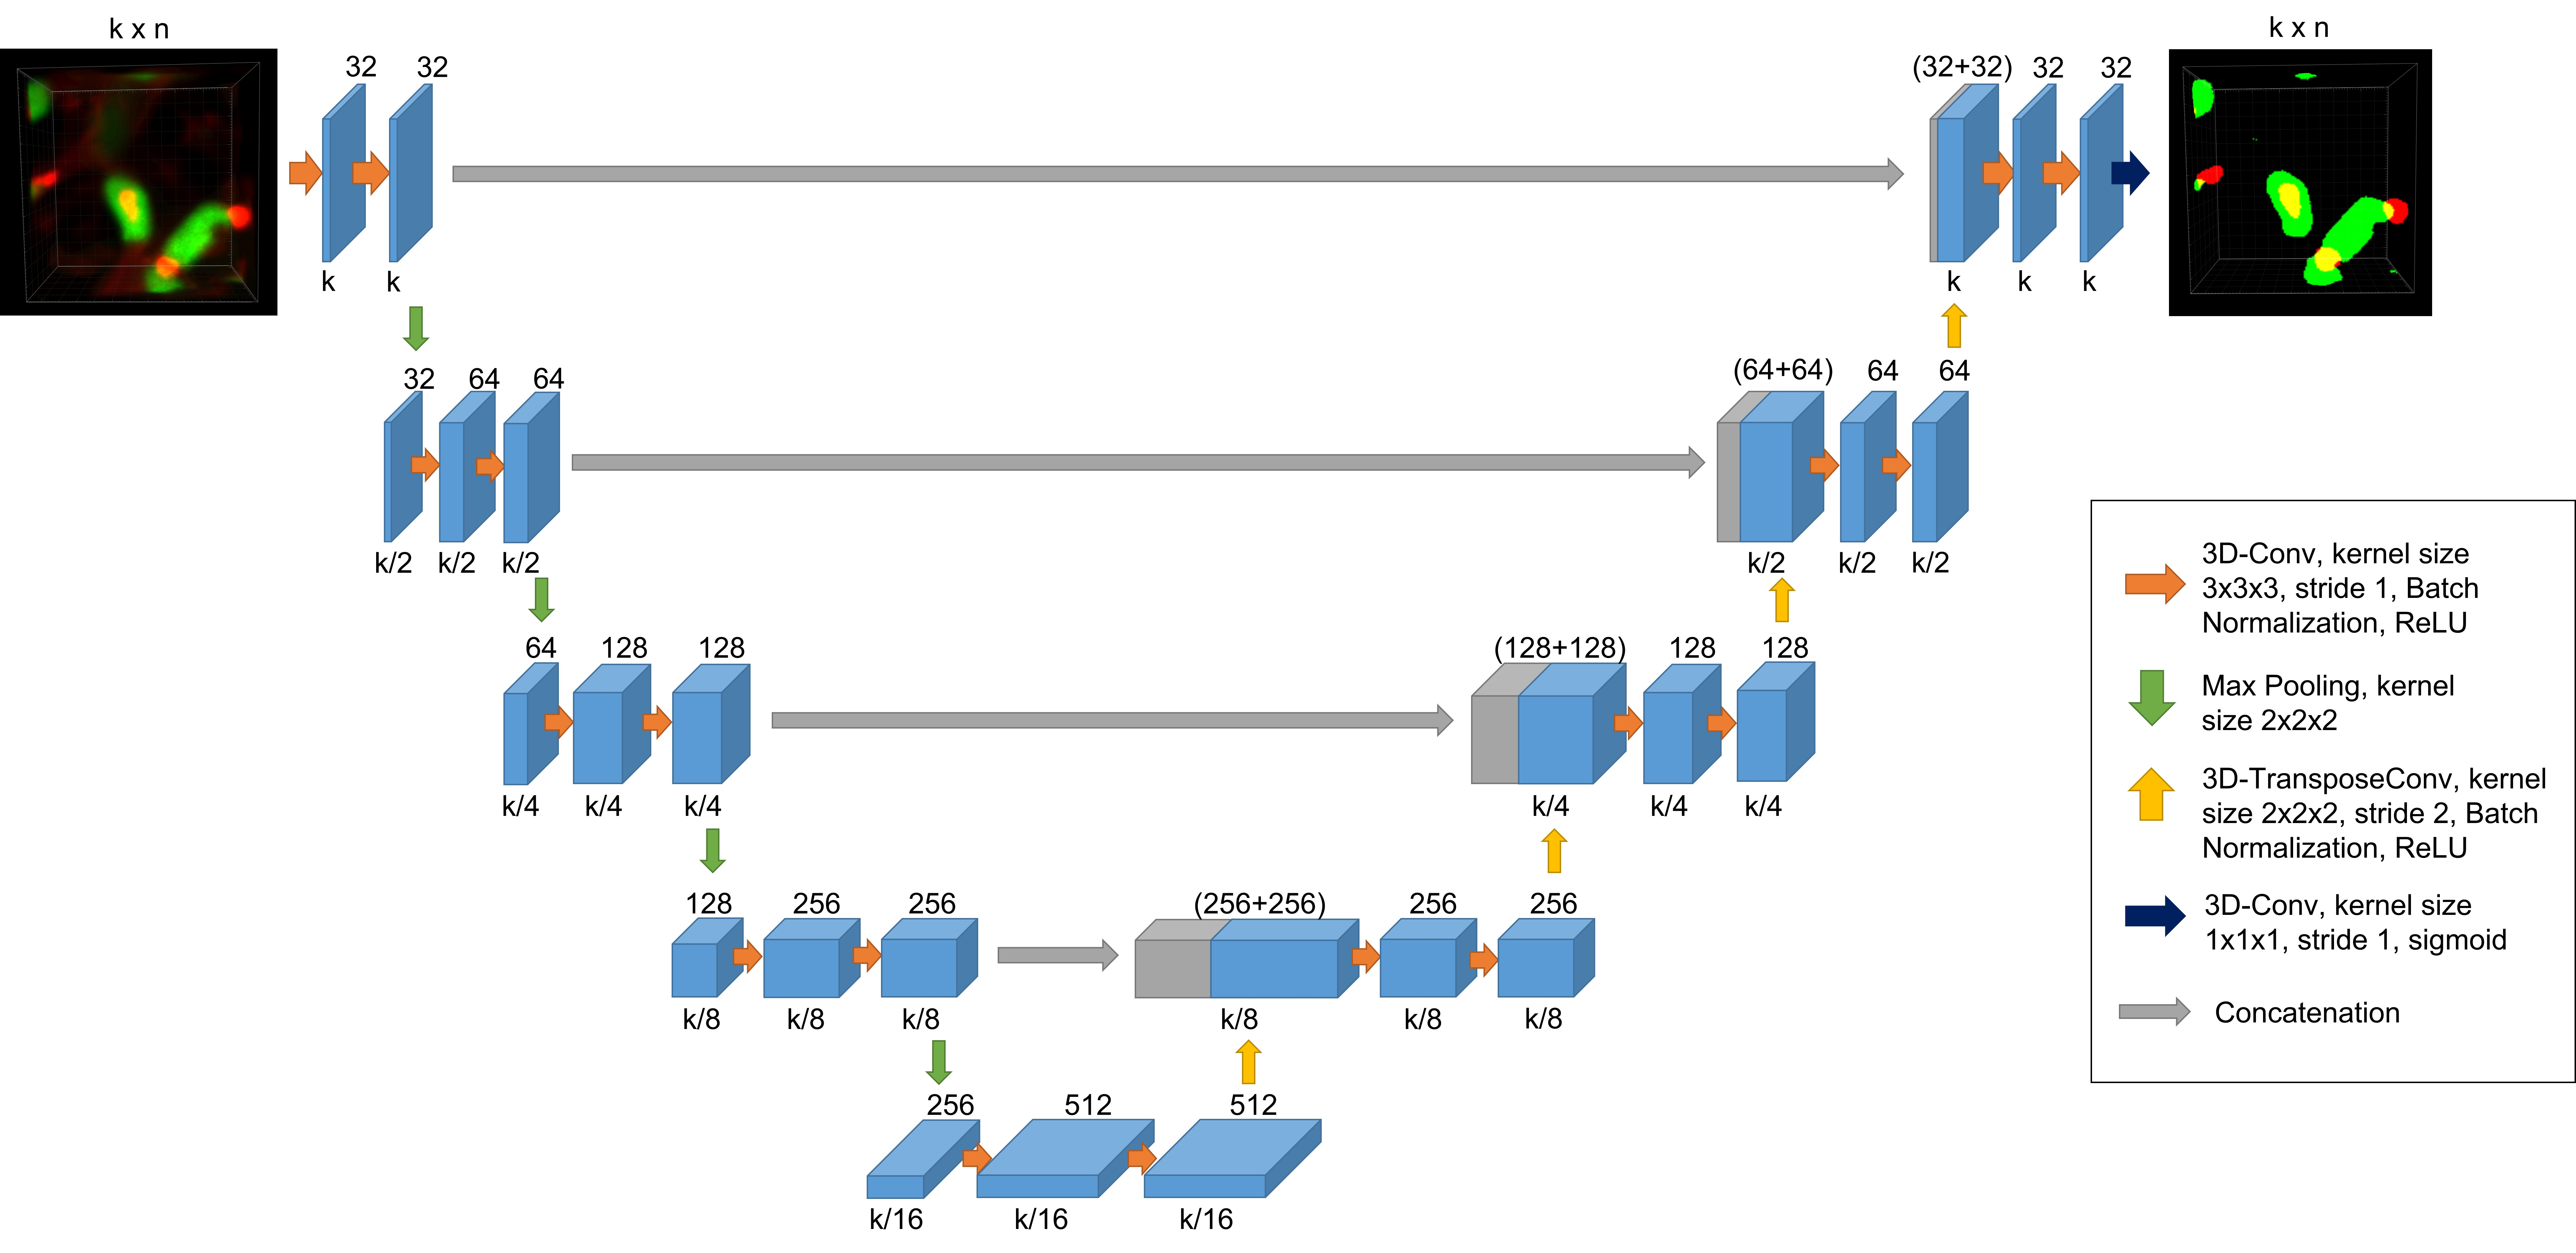
\includegraphics[width=0.85\textwidth]{Images/Picture1.jpg}
  \caption{Implemented \ac{3D} U-Net architecture. $k=(x,y,z)$ denotes the size of the input image for the x, y and z axes. $n$ denores the number of input/output channels.}
  \label{fig:y-unet-3d}
\end{figure}

In the Figure above, each blue box corresponds to a multi-channel feature map. The number of channels is indicated at the top of the box. The size of the feature map is provided at the bottom of the box with respect to the size of the input image $k$. Grey boxes represent copied feature maps. The arrows denote the different operations. The $n$ (above the input and output images) is the number of channels of the input and output images, $n$=2 and $n$=3 for the 2-class and 3-class segmentation tasks, respectively. The output image in the Figure is an example of the output for the 2-class segmentation task.

The \ac{DC} is a widely used metric in the computer vision community to calculate the similarity between two images \cite{diceloss}. Therefore, the dice coefficient has been fitted to a loss function known as \ac{DLoss}:

\begin{equation}
    DLoss(y,\hat{p}) = 1 - \frac{2y\hat{p}+1}{y+\hat{p}+1}
    \label{eq:dice-loss}
\end{equation}

\noindent here $y$ is the reference value, $\hat{p}$ is the probability value predicted by the model and 1 is added to both the numerator and denominator to ensure that the function is not undefined in edge case scenarios, e.g., when $y=\hat{p}=0$. Unlike the original \ac{3D} U-Net model \cite{Unet:3D} previously described in Section \ref{section:CNN&UNET}, the loss function used in training the model is the Dice loss represented in equation \ref{eq:dice-loss}.

\subsection{Vox2Vox}

Pix2Pix is a supervised GAN model designed for image-to-image translation, previously described in subsection \ref{subsection:pix2pix}. However, it is not capable of performing image-to-image translation at the \ac{3D} level. A \ac{3D} volume-to-volume network for segmentation used as an alternative to Pix2Pix is the Vox2Vox network.

\citet{vox2vox} used a Vox2Vox approach in their work. For this work, it will be used a similar architecture. The generator model is built in the style of the U-Net and Res-Net \cite{2015deep} architectures, while the discriminator is built in the style of the PatchGAN \cite{isola2018imagetoimage}  architecture. The implemented architectures are shown in Figures \ref{fig:genvox} and \ref{fig:discvox}.

\begin{figure}[!htb]
  \centering
  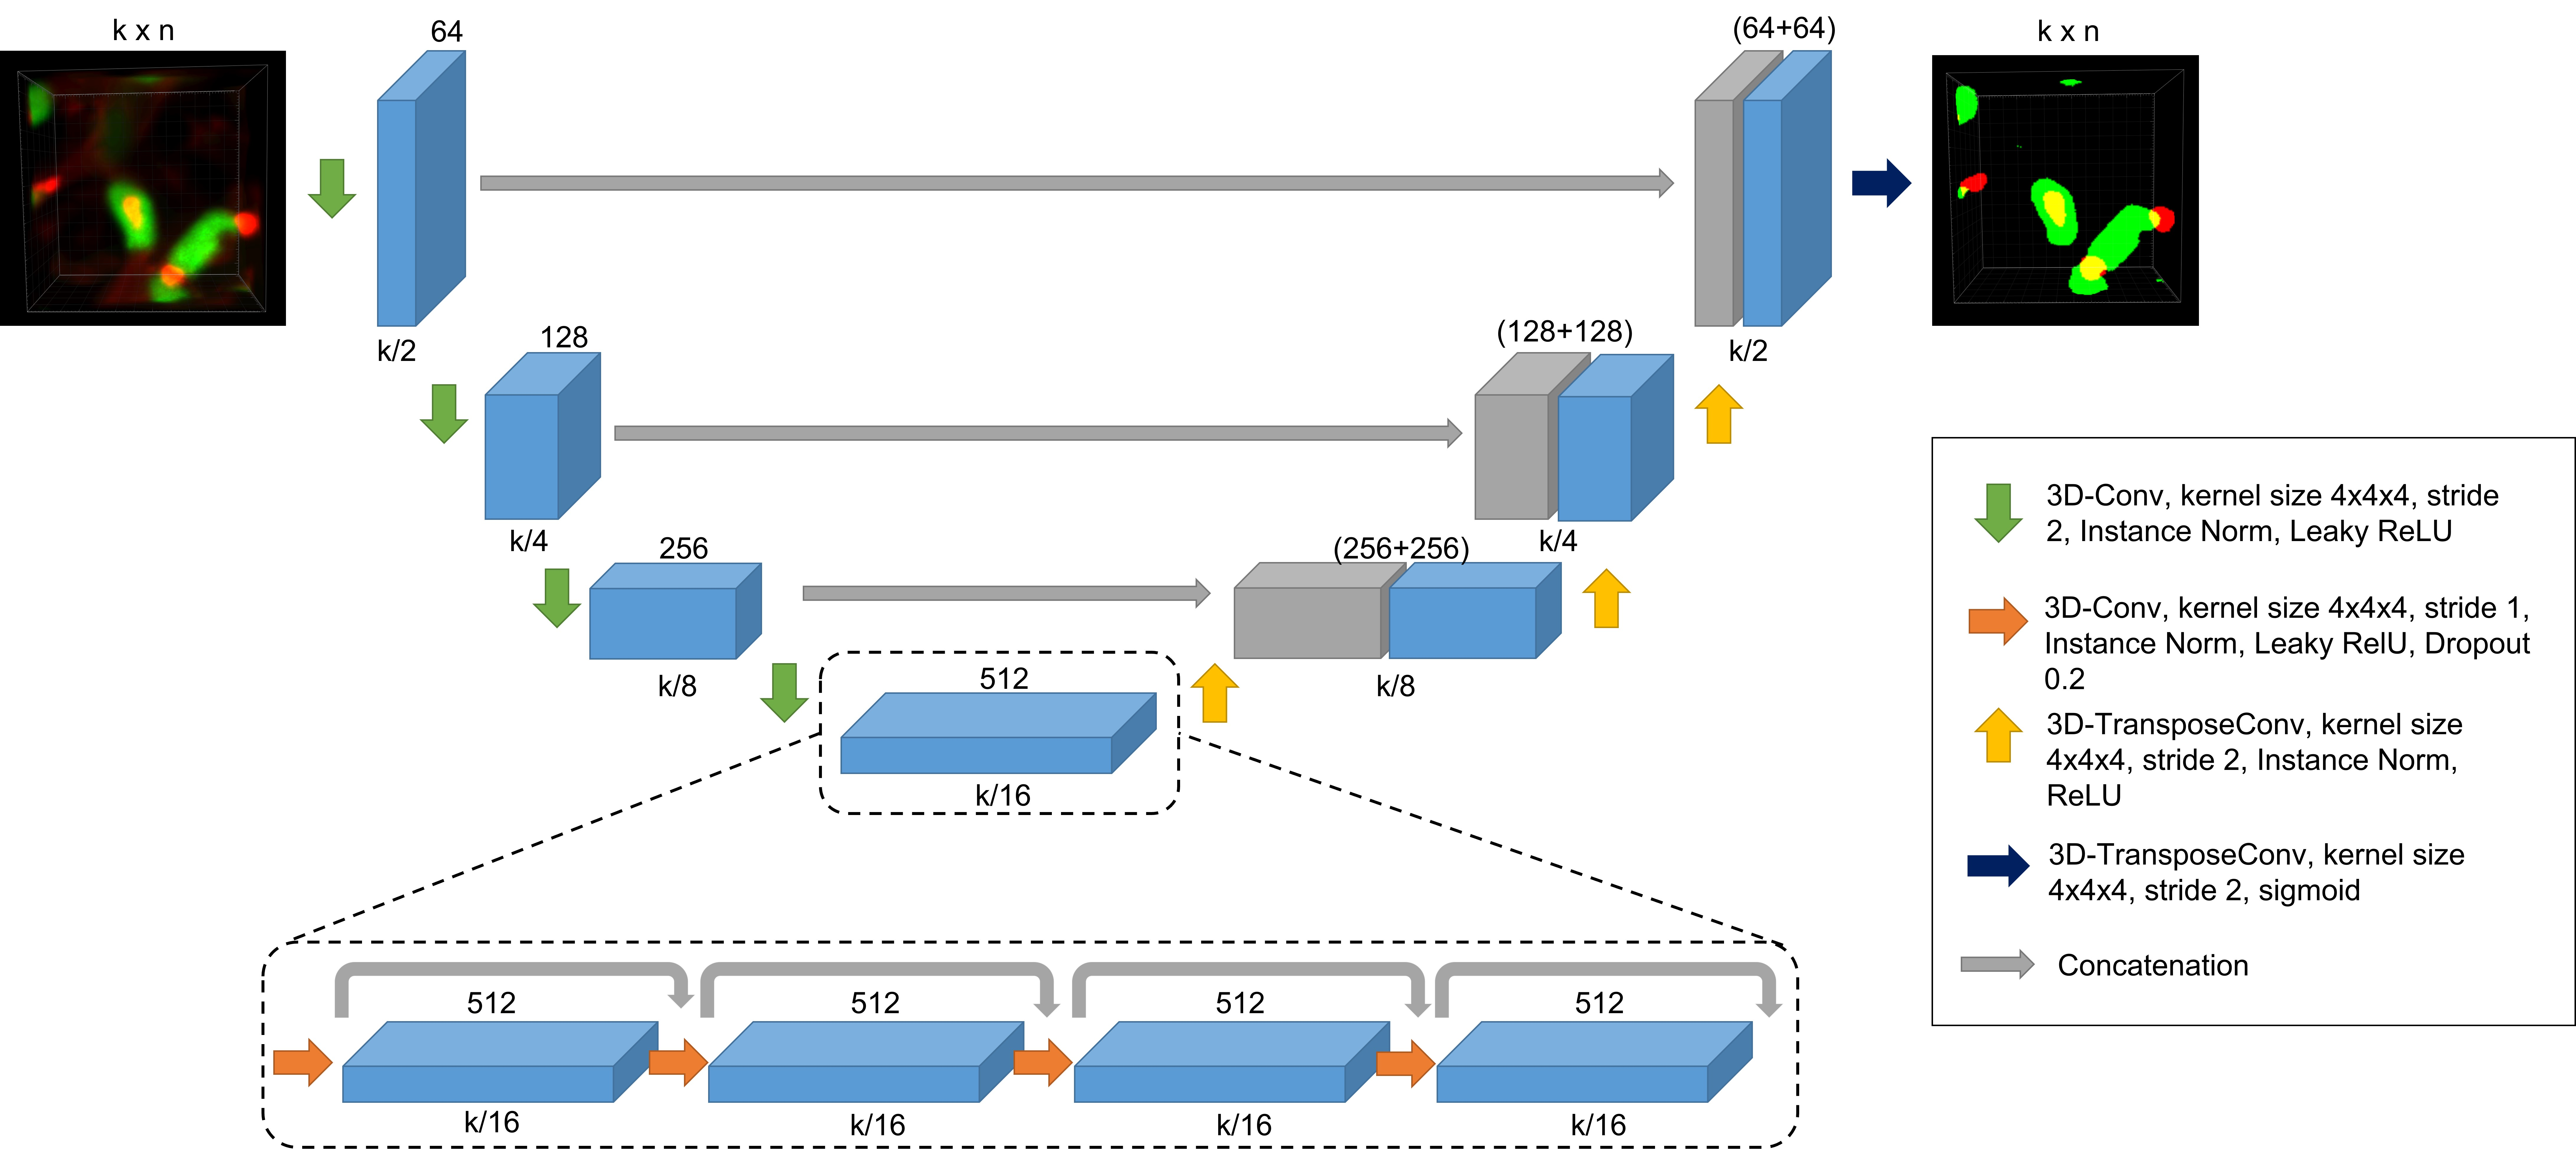
\includegraphics[width=0.85\textwidth]{Images/Picture2.jpg}
  \caption[Implemented Vox2Vox generator architecture.]{Implemented Vox2Vox generator architecture. $k=(x,y,z)$ denotes the size of the input image for the x, y and z axes. $n$ denores the number of input/output channels.}
  \label{fig:genvox}
\end{figure}

\begin{figure}[!htb]
  \centering
  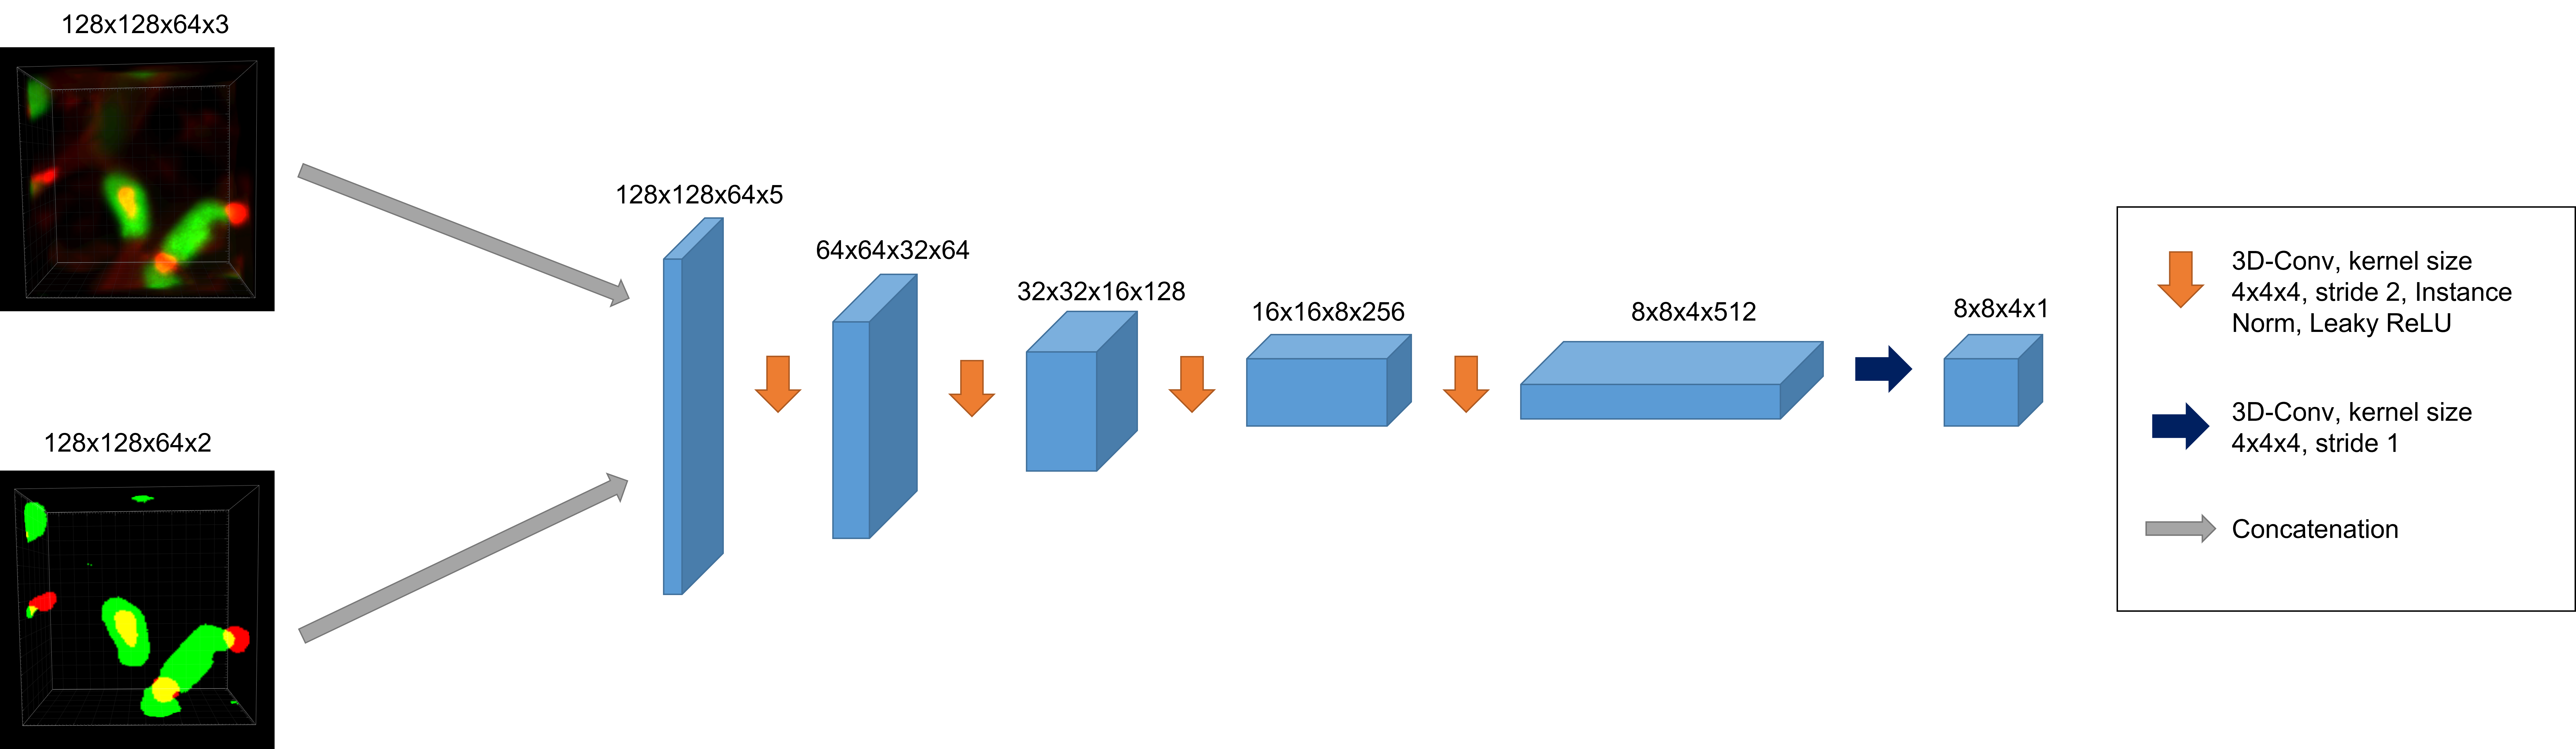
\includegraphics[width=0.90\textwidth]{Images/discriminator_vox.jpg}
  \caption[Implemented Vox2Vox discriminator architecture.]{Implemented Vox2Vox discriminator architecture. $k=(x,y,z)$ denotes the size of the input image for the x, y and z axes. $n$ denores the number of input/output channels.}
  \label{fig:discvox}
\end{figure}

In the Figures \ref{fig:genvox} and \ref{fig:discvox}, each blue box corresponds to a multi-channel feature map. The number of channels is indicated at the top of the box. The size of the feature map is provided at the bottom of the box with respect to the size of the input image $k$. Grey boxes represent copied feature maps. The arrows denote the different operations. The $n$ (above the input and output images in the generator architecture) is the number of channels of the input and output images. The output of the generator architecture is an example of the output for the 2-class segmentation task.

Another important part of the implementation of Vox2Vox model is the loss function. The discriminator loss, $\mathcal{L}_{disc}$, is the sum of the $L_2$ error of the discriminator output between the original image $x$ and the respective ground-truth $y$ with a tensor of ones, and the $L_2$ error of the discriminator output between the original image and the respective segmentation prediction $\hat{y}$ given by the generator with a tensor of zeros. This can be formulated as follows:

\begin{equation}
    \mathcal{L}_{disc} = L_2[D(x,y),\boldsymbol{1}] + L_2[D(x,\hat{y}),\boldsymbol{0}].
\end{equation}

On the other hand, the generator loss, $\mathcal{L}_{gen}$, is the sum of the $L_2$ error of the discriminator output between the original image, $x$, and the corresponding segmentation prediction, $\hat{y}$, with a tensor of ones, and the \ac{DLoss}, between the ground-truth and the generator output multiplied by the scalar weight coefficient $\alpha > 0$. This can be formulated in the following way:

\begin{equation}
\label{eq:vox2vox-generator-loss}
    \mathcal{L}_{gen} = L_2[D(x,\hat{y}),\boldsymbol{1}] + \alpha DLoss(y,\hat{y}).
\end{equation}

\section{Models Inference}
\label{section:models_inference}

As indicated in Section \ref{section:dataset}, the input size of the proposed models is 64x64x64. Therefore, to obtain the predicted segmentation mask of an entire crop, it is necessary to slide a \ac{3D} window of size 64x64x64 to segment the entire crop. To make the segmentation mask the same size as the original crop, we need to pad the X and Y axes of the original image so that the dimensions are $X_{pad} = (X \% step) \times step $ and $Y_{pad} = (Y \% step) \times step $, where $step$ is the number of pixels the \ac{3D} window moves during inference. The padding used is reflection padding. If you place a \ac{3D} window in the upper left corner of the padded crop a 64x64x64 patch becomes the input volume of the model used to create a sub-volume of the segmentation mask in the upper left. This \ac{3D} window is slid in x and y direction with a certain $step$ through the entire padded crop until the entire volume is processed.



\section{Execution time}
\label{section:execution_time}

The execution time of a deep neural network model can be divided into two intervals: the training time and the testing time. Here, the training time corresponds to the time it takes for a model to learn a particular task. The test time is the time required for a model to make a segmentation prediction for an image. In this work, the execution time is also considered as a measure of the performance of the different approaches. For supervised methods that require manual annotations, the time required to create these masks is also considered.